\documentclass[border=4pt]{standalone}
% Shared style for the workflow figures (standalone TikZ, compiled to PDF).
\usepackage[T1]{fontenc}
\usepackage[scaled=0.95]{helvet}
\renewcommand{\familydefault}{\sfdefault}
\usepackage{amsmath,amssymb}
\usepackage{xcolor}
\usepackage{tikz}
\usetikzlibrary{arrows.meta,positioning,calc,fit,backgrounds,shapes.misc,shapes.geometric}

\definecolor{cBlue}{HTML}{2B6CB0}
\definecolor{cTeal}{HTML}{1C8C8C}
\definecolor{cGreen}{HTML}{2F855A}
\definecolor{cPurple}{HTML}{6B46C1}
\definecolor{cOrange}{HTML}{C05621}
\definecolor{cRed}{HTML}{C53030}
\definecolor{cGray}{HTML}{4A5568}
\definecolor{cInk}{HTML}{1A202C}

\tikzset{
  cardbody/.style={rectangle, rounded corners=3pt, line width=0.9pt, align=left,
                   font=\scriptsize\color{cInk}, inner xsep=5pt, inner ysep=5pt},
  cardhead/.style={rectangle, rounded corners=3pt, align=left, text=white,
                   font=\footnotesize, inner xsep=4pt, inner ysep=3.5pt},
  numc/.style={circle, line width=0.9pt, inner sep=0pt, minimum size=5.2mm,
               font=\footnotesize\bfseries},
  flow/.style={-{Stealth[length=2.6mm,width=2.2mm]}, line width=1.3pt, color=cGray},
  loop/.style={-{Stealth[length=2.4mm,width=2mm]}, line width=1.1pt, dashed, color=cRed},
  tag/.style={rectangle, rounded corners=2pt, font=\scriptsize\bfseries, inner sep=2.5pt},
  note/.style={font=\scriptsize\itshape, color=cGray, align=center},
  band/.style={rectangle, rounded corners=6pt, line width=0.8pt, inner sep=7pt},
}

% \card{name}{position}{colour}{number}{title}{body}{width}{body height}
\newcommand{\card}[8]{%
  \node[cardbody, draw=#3, fill=#3!5, text width=#7, minimum height=#8, anchor=north]
       (#1) at (#2) {#6};
  \node[cardhead, fill=#3, text width=#7, anchor=south, yshift=-1.5pt] (#1h) at (#1.north) {\hspace*{4.2mm}\textbf{#5}};
  \node[numc, fill=white, draw=#3, text=#3] at ([xshift=1pt]#1h.west) {#4};
}
\newcommand{\bul}{\textcolor{cGray}{\textbullet}~}

\begin{document}
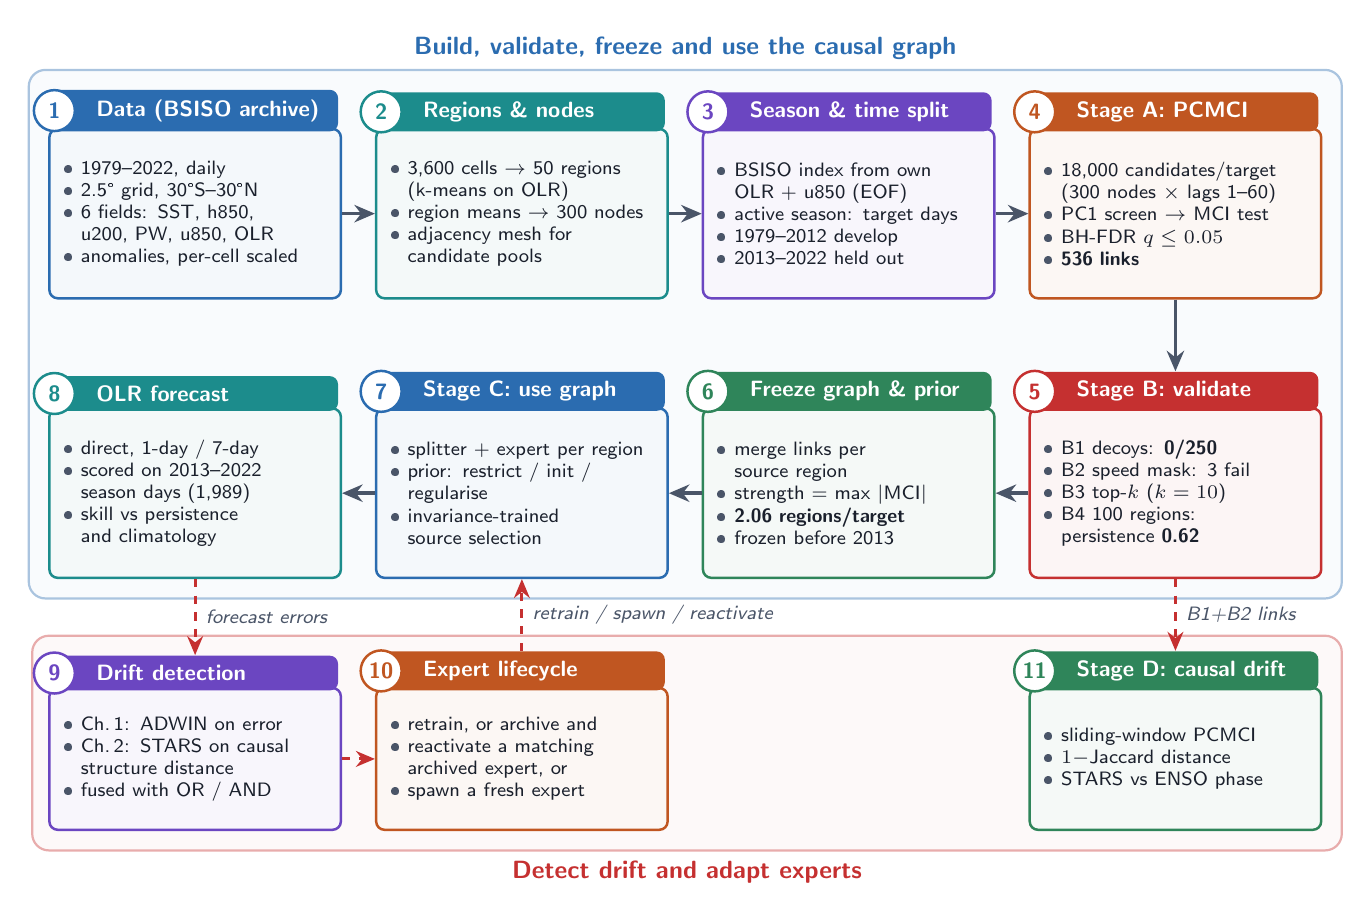
\begin{tikzpicture}
\def\W{3.35cm}\def\H{2.15cm}
\def\dx{4.15}
% ---- row 1
\card{c1}{0,0}{cBlue}{1}{Data (BSISO archive)}{\bul 1979--2022, daily\\\bul 2.5\textdegree\ grid, 30\textdegree S--30\textdegree N\\\bul 6 fields: SST, h850,\\\hphantom{\bul}u200, PW, u850, OLR\\\bul anomalies, per-cell scaled}{\W}{\H}
\card{c2}{\dx,0}{cTeal}{2}{Regions \& nodes}{\bul 3{,}600 cells $\rightarrow$ 50 regions\\\hphantom{\bul}(k-means on OLR)\\\bul region means $\rightarrow$ 300 nodes\\\bul adjacency mesh for\\\hphantom{\bul}candidate pools}{\W}{\H}
\card{c3}{2*\dx,0}{cPurple}{3}{Season \& time split}{\bul BSISO index from own\\\hphantom{\bul}OLR + u850 (EOF)\\\bul active season: target days\\\bul 1979--2012 develop\\\bul 2013--2022 held out}{\W}{\H}
\card{c4}{3*\dx,0}{cOrange}{4}{Stage A: PCMCI}{\bul 18{,}000 candidates/target\\\hphantom{\bul}(300 nodes $\times$ lags 1--60)\\\bul PC1 screen $\rightarrow$ MCI test\\\bul BH-FDR $q\le0.05$\\\bul \textbf{536 links}}{\W}{\H}
% ---- row 2 (right to left)
\card{c5}{3*\dx,-3.55}{cRed}{5}{Stage B: validate}{\bul B1 decoys: \textbf{0/250}\\\bul B2 speed mask: 3 fail\\\bul B3 top-$k$ ($k=10$)\\\bul B4 100 regions:\\\hphantom{\bul}persistence \textbf{0.62}}{\W}{\H}
\card{c6}{2*\dx,-3.55}{cGreen}{6}{Freeze graph \& prior}{\bul merge links per\\\hphantom{\bul}source region\\\bul strength = max $|$MCI$|$\\\bul \textbf{2.06 regions/target}\\\bul frozen before 2013}{\W}{\H}
\card{c7}{\dx,-3.55}{cBlue}{7}{Stage C: use graph}{\bul splitter + expert per region\\\bul prior: restrict / init /\\\hphantom{\bul}regularise\\\bul invariance-trained\\\hphantom{\bul}source selection}{\W}{\H}
\card{c8}{0,-3.55}{cTeal}{8}{OLR forecast}{\bul direct, 1-day / 7-day\\\bul scored on 2013--2022\\\hphantom{\bul}season days (1{,}989)\\\bul skill vs persistence\\\hphantom{\bul}and climatology}{\W}{\H}
% ---- row 3 (adaptation)
\card{c9}{0,-7.1}{cPurple}{9}{Drift detection}{\bul Ch.\,1: ADWIN on error\\\bul Ch.\,2: STARS on causal\\\hphantom{\bul}structure distance\\\bul fused with OR / AND}{\W}{1.8cm}
\card{c10}{\dx,-7.1}{cOrange}{10}{Expert lifecycle}{\bul retrain, or archive and\\\bul reactivate a matching\\\hphantom{\bul}archived expert, or\\\bul spawn a fresh expert}{\W}{1.8cm}
\card{c11}{3*\dx,-7.1}{cGreen}{11}{Stage D: causal drift}{\bul sliding-window PCMCI\\\bul $1-$Jaccard distance\\\bul STARS vs ENSO phase}{\W}{1.8cm}
% ---- arrows
\foreach \a/\b in {c1/c2,c2/c3,c3/c4}{\draw[flow] (\a.east) -- (\b.west);}
\draw[flow] (c4.south) -- (c5h.north);
\foreach \a/\b in {c5/c6,c6/c7,c7/c8}{\draw[flow] (\a.west) -- (\b.east);}
\draw[loop] (c8.south) -- node[note, right]{forecast errors} (c9h.north);
\draw[loop] (c9.east) -- (c10.west);
\draw[loop] (c10h.north) -- node[note, right]{retrain / spawn / reactivate} (c7.south);
\draw[loop] (c5.south) -- node[note, right]{B1+B2 links} (c11h.north);
% ---- bands
\begin{scope}[on background layer]
\node[band, draw=cBlue!40, fill=cBlue!3, fit=(c1h)(c4)(c5)(c8), label={[font=\small\bfseries\color{cBlue}]above:Build, validate, freeze and use the causal graph}] {};
\node[band, draw=cRed!40, fill=cRed!3, fit=(c9h)(c11), label={[font=\small\bfseries\color{cRed}]below:Detect drift and adapt experts}] {};
\end{scope}
\end{tikzpicture}
\end{document}
